Table~\ref{tab:primary} reports the fixed-realization comparison. IGRB selects nonzero graph corrections for seasonal and correlated demand and returns exactly to the local expert for intermittent and retail-driven demand. The graph contribution is selective by construction.
\begin{table}[tb]\centering\scriptsize
\caption{Unchanged-condition predictive results on the fixed benchmark realization (mean over five model seeds). RMSE$^+$ is normalized severity RMSE on positive targets.}\label{tab:primary}
\resizebox{\linewidth}{!}{\begin{tabular}{lrrrrrr}\toprule Case & Method & Macro F1 & AP & Brier & RMSE$^+$ & $\alpha$ \\\midrule
Seasonal & Local expert & 0.6752 & 0.4769 & 0.1138 & 0.4445 & 0.00 \\
Seasonal & IGRB & 0.6804 & 0.4852 & 0.1128 & 0.4415 & 0.68 \\
\addlinespace
Intermittent & Local expert & 0.6939 & 0.7902 & 0.1926 & 2.0331 & 0.00 \\
Intermittent & IGRB & 0.6939 & 0.7902 & 0.1926 & 2.0331 & 0.00 \\
\addlinespace
Correlated & Local expert & 0.7832 & 0.8801 & 0.1426 & 1.0458 & 0.00 \\
Correlated & IGRB & 0.7953 & 0.8899 & 0.1388 & 1.1139 & 0.52 \\
\addlinespace
Retail-driven & Local expert & 0.8611 & 0.9574 & 0.1047 & 8.6768 & 0.00 \\
Retail-driven & IGRB & 0.8611 & 0.9574 & 0.1047 & 8.6768 & 0.00 \\
\addlinespace
\bottomrule\end{tabular}}\end{table}
Figure~\ref{fig:fixed} visualizes the two occurrence metrics. In seasonal demand, the correction raises macro F1 by 0.0051 and AP by 0.0083 while slightly lowering Brier score and RMSE$^+$. In correlated demand, it raises macro F1 by 0.0120 and AP by 0.0098 and lowers Brier score by 0.0038, but RMSE$^+$ increases by 0.0681. The latter is an important counter-result: the contextual correction improves occurrence prediction without uniformly improving conditional quantity estimates. Exact equality in the intermittent and retail-driven panels follows from $\alpha=0$, not rounding of distinct models.
\begin{figure}[tb]\centering
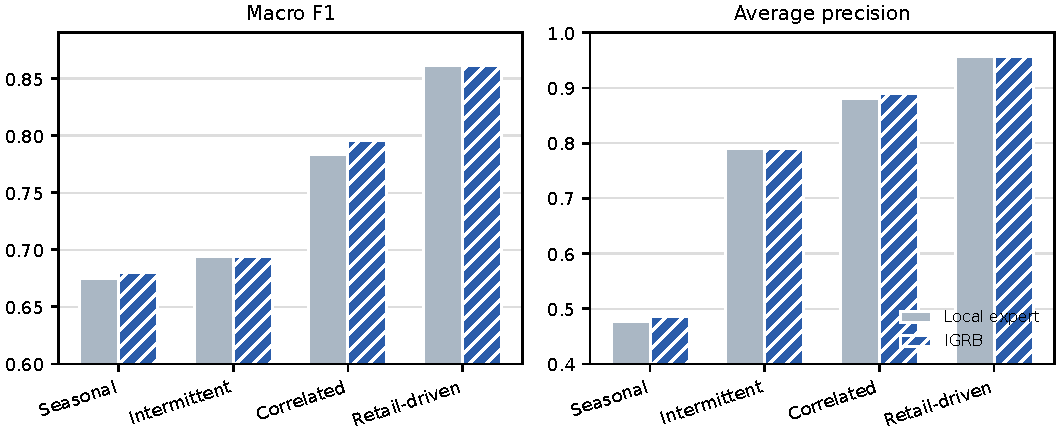
\includegraphics[width=.96\linewidth]{igrb_fixed_performance.pdf}
\caption{Fixed-realization occurrence performance, averaged over five model seeds. Exact ties occur where the intermittency screen returns IGRB to the local expert.}\label{fig:fixed}
\end{figure}

The independently sourced FMCG-inspired panel is reported separately because its source is simulated and only three parsimonious benchmark controls were rerun. IGRB improves over its tuned local expert but does not exceed standard XGBoost on macro F1. Its lower positive-severity RMSE shows a different occurrence--quantity trade-off rather than universal superiority.
\begin{table}[tb]\centering\small
\caption{FMCG-inspired robustness check under the unchanged condition (mean $\pm$ standard deviation over five model seeds; deterministic controls have zero standard deviation).}\label{tab:fmcg}
\begin{tabular}{lrrrr}\toprule Method & Macro F1 & AP & Brier & RMSE$^+$ \\\midrule
Local balance & $0.3682\pm0.0000$ & 0.1777 & 0.3998 & 12.0218 \\
Persistence & $0.7251\pm0.0000$ & 0.3392 & 0.1294 & 0.6154 \\
XGBoost & $0.7608\pm0.0003$ & 0.6345 & 0.0732 & 0.7799 \\
Tuned local expert & $0.7573\pm0.0025$ & 0.6322 & 0.0736 & 0.7376 \\
IGRB & $0.7592\pm0.0013$ & 0.6329 & 0.0737 & 0.6903 \\
\bottomrule\end{tabular}\end{table}
Against the strongest benchmark comparator, IGRB improves macro F1 in seasonal, intermittent and correlated demand and is practically tied in retail-driven demand. The intermittent gain is attributable to the retuned local expert because graph correction is disabled.
\begin{table}[tb]\centering\small
\caption{IGRB versus the strongest benchmark comparator, unchanged fixed realization.}\label{tab:previous}
\begin{tabular}{llrrr}\toprule Case & Previous best & Previous F1 & IGRB F1 & Difference \\\midrule
Seasonal & RelGRU & 0.6413 & 0.6804 & +0.0391 \\
Intermittent & LSTM & 0.6819 & 0.6939 & +0.0121 \\
Correlated & XGBoost & 0.7859 & 0.7953 & +0.0094 \\
Retail-driven & XGBoost & 0.8613 & 0.8611 & -0.0002 \\
\bottomrule\end{tabular}\end{table}
This comparison separates graph-specific gains from improvements in the local model. In seasonal and correlated demand, IGRB adds a nonzero graph correction and exceeds the strongest comparator by 0.0391 and 0.0094, respectively. In intermittent demand, its 0.0121 advantage over the strongest comparator comes entirely from the tuned local XGBoost reference. In retail-driven demand, the difference from the strongest XGBoost result is $-0.0002$, which is practically negligible and supplies no evidence of superiority.

Figure~\ref{fig:allbaselines} reports the complete fixed-realization comparison rather than only the strongest comparator. IGRB has the highest displayed mean in seasonal and correlated demand, ties its tuned local expert in intermittent demand, and is practically tied with both local XGBoost variants in the retail-driven case. The comparison also shows why the tuned local expert is a necessary reference: it is substantially stronger than several neural graph models, particularly on the retail-derived streams. Red outlines mark the column maximum or values within $5\times10^{-4}$ of it; they are descriptive fixed-record rankings, not significance claims.

\begin{figure}[tb]\centering
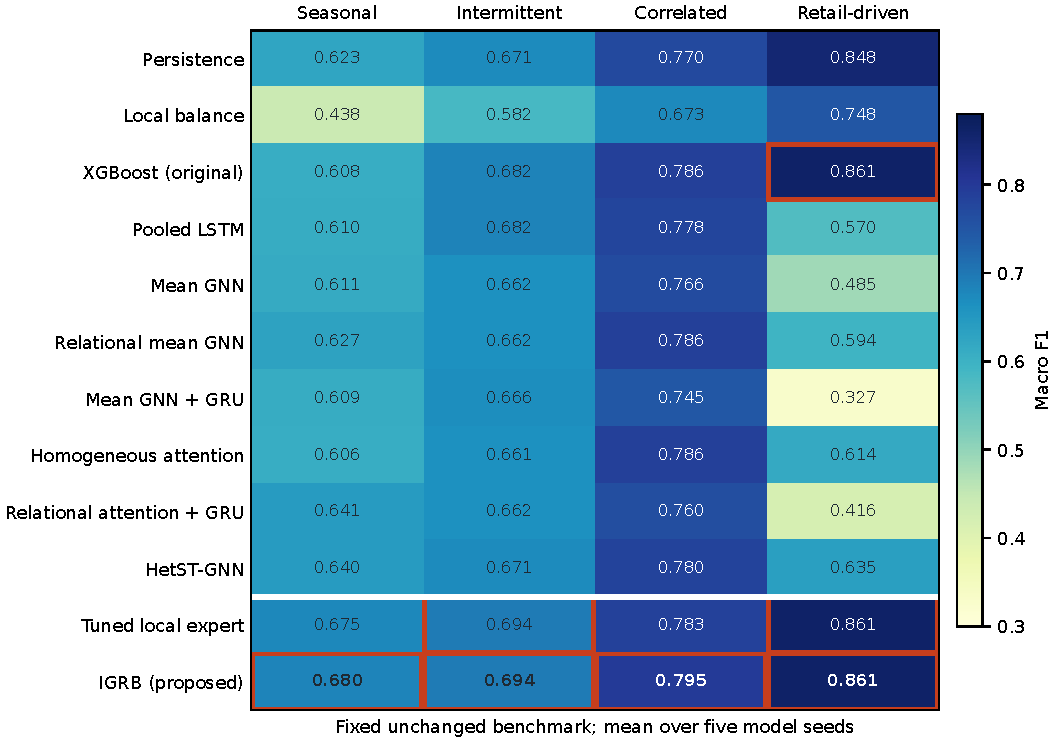
\includegraphics[width=.96\linewidth]{igrb_all_baselines.pdf}
\caption{Complete unchanged-condition macro-F1 comparison on the fixed benchmark realization. The first ten rows are benchmark methods; the last two rows are the tuned local reference and IGRB. Values are means over five model seeds, except deterministic controls. Red outlines denote the column maximum or a practical tie within 0.0005.}\label{fig:allbaselines}
\end{figure}
Independent records provide the stronger generalization check (Table~\ref{tab:independent}). The unchanged correlated-demand interval excludes zero across ten records; the seasonal interval crosses zero after five additional records are included. Intermittent demand is an exact fallback.
\begin{table}[tb]\centering\small
\caption{Paired IGRB minus local-expert macro-F1 differences over independent demand replications; percentile bootstrap intervals use 30,000 paired resamples.}\label{tab:independent}
\begin{tabular}{llrrrrr}\toprule Case & Condition & $n$ & Difference & 95\% interval & Wins & Losses \\\midrule
Seasonal & Unchanged & 10 & +0.0033 & [-0.0028, +0.0089] & 7 & 3 \\
Seasonal & Lead-time shift & 10 & -0.0087 & [-0.0278, +0.0087] & 4 & 6 \\
Seasonal & Policy shift & 10 & -0.0082 & [-0.0276, +0.0088] & 5 & 5 \\
\addlinespace
Intermittent & Unchanged & 5 & +0.0000 & [+0.0000, +0.0000] & 0 & 0 \\
Intermittent & Lead-time shift & 5 & +0.0000 & [+0.0000, +0.0000] & 0 & 0 \\
Intermittent & Policy shift & 5 & +0.0000 & [+0.0000, +0.0000] & 0 & 0 \\
\addlinespace
Correlated & Unchanged & 10 & +0.0269 & [+0.0080, +0.0436] & 9 & 1 \\
Correlated & Lead-time shift & 10 & +0.0149 & [-0.0083, +0.0358] & 8 & 2 \\
Correlated & Policy shift & 10 & +0.0228 & [+0.0094, +0.0420] & 9 & 1 \\
\addlinespace
\bottomrule\end{tabular}\end{table}
\begin{figure}[tb]\centering
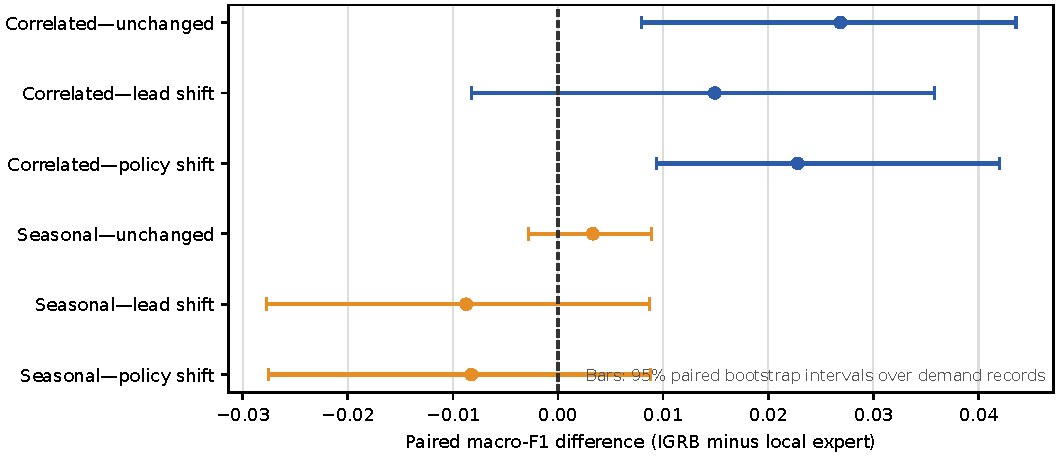
\includegraphics[width=.96\linewidth]{igrb_independent_effects.pdf}
\caption{Record-level paired effects after averaging five model seeds within each demand realization. The vertical reference is no difference; intervals are percentile paired-bootstrap intervals.}\label{fig:independent}
\end{figure}
The record-level evidence materially changes the conclusion suggested by the fixed benchmark. For unchanged correlated demand, the mean gain is 0.0269, nine of ten records favor IGRB and the interval remains above zero. Under the policy shift, nine of ten records also favor IGRB and the interval is positive. Under the lead-time shift, eight of ten favor it, but two adverse records widen the interval across zero. The appropriate claim is therefore robustness to unchanged and policy-shifted correlated demand, with uncertainty under longer transit time.

Seasonal demand is less stable. Seven of ten unchanged records favor IGRB, yet the mean gain is only 0.0033 and the interval spans zero. Under both shifts, the mean difference is negative and the intervals again span zero. The first five records were more favorable; the next five remove a broad seasonal-superiority conclusion. This is why demand-record uncertainty is reported separately from the small standard deviations over model seeds.
The component study in Table~\ref{tab:ablation} shows that forcing the graph expert harms intermittent demand and removing the ADI screen reduces its mean F1. Graph-only is slightly higher in the fixed dense cases, but it removes the fallback protection and its advantage is not evidence of general robustness. Error weighting is not uniformly beneficial and is excluded from the final method.
\begin{table}[tb]\centering\scriptsize
\caption{Component ablations on the unchanged fixed realization (mean $\pm$ standard deviation over five model seeds).}\label{tab:ablation}
\resizebox{\linewidth}{!}{\begin{tabular}{lrrrr}\toprule Case & Local only & Graph only & IGRB & Targeted ablation \\\midrule
Seasonal & 0.6752 $\pm$ 0.0035 & 0.6808 $\pm$ 0.0043 & 0.6804 $\pm$ 0.0037 & Error-weighted: 0.6808 $\pm$ 0.0050 \\
Intermittent & 0.6939 $\pm$ 0.0045 & 0.6851 $\pm$ 0.0035 & 0.6939 $\pm$ 0.0045 & No ADI: 0.6886 $\pm$ 0.0028 \\
Correlated & 0.7832 $\pm$ 0.0103 & 0.8051 $\pm$ 0.0084 & 0.7953 $\pm$ 0.0090 & Error-weighted: 0.7932 $\pm$ 0.0140 \\
Retail-driven & 0.8611 $\pm$ 0.0022 & 0.8625 $\pm$ 0.0013 & 0.8611 $\pm$ 0.0022 & No ADI: 0.8623 $\pm$ 0.0024 \\
\bottomrule\end{tabular}}\end{table}
The ablation also exposes the cost of a conservative method. Graph-only is 0.0099 above IGRB in the fixed correlated case and 0.0005 above it in seasonal demand. A method optimized solely for these two cells might therefore omit shrinkage and fallback. However, graph-only loses 0.0088 relative to local-only under intermittent demand, and the no-ADI variant also loses 0.0053 there. The selected design favors bounded downside across regimes over maximizing the best dense-case point estimate. In retail-driven demand, graph-only and no-ADI are slightly above the fallback point estimate, but the pre-specified ADI rule intentionally declines to treat that tiny fixed-record difference as sufficient evidence.

Table~\ref{tab:adi-sensitivity} tests whether this conclusion is an artifact of the borrowed 1.32 boundary. Cutoffs from 1.20 to 1.50 produce the same activation pattern and the same fixed-record results: graph correction is admitted for seasonal, correlated and FMCG-inspired demand and rejected for retail-driven and intermittent demand. A cutoff of 1.00 is too strict to admit the correlated and FMCG-inspired cases because their training ADIs are 1.007 and 1.143. At 2.00, the retail correction is admitted and adds only 0.0012 macro F1; intermittent demand, with ADI 2.549, still falls back. The analysis therefore supports a stable operating region rather than claiming that 1.32 is uniquely optimal.

\begin{table}[tb]\centering\scriptsize
\caption{Sensitivity of fixed-realization macro-F1 differences (selected framework minus local expert) to the ADI cutoff. S, C, F, R and I denote seasonal, correlated, FMCG-inspired, retail-driven and intermittent demand.}\label{tab:adi-sensitivity}
\resizebox{\linewidth}{!}{\begin{tabular}{lcrrrrr}\toprule
ADI cutoff & Graph-active cases & $\Delta$F1 S & $\Delta$F1 C & $\Delta$F1 F & $\Delta$F1 R & $\Delta$F1 I \\\midrule
1.00 & S & +0.0051 & +0.0000 & +0.0000 & +0.0000 & +0.0000 \\
1.20 & S, C, F & +0.0051 & +0.0120 & +0.0018 & +0.0000 & +0.0000 \\
1.32 & S, C, F & +0.0051 & +0.0120 & +0.0018 & +0.0000 & +0.0000 \\
1.50 & S, C, F & +0.0051 & +0.0120 & +0.0018 & +0.0000 & +0.0000 \\
2.00 & S, C, F, R & +0.0051 & +0.0120 & +0.0018 & +0.0012 & +0.0000 \\
\bottomrule\end{tabular}
}
\end{table}

The central operational result is the decision guardrail's selectivity, not the magnitude of one cost percentage. It abstains in seasonal, intermittent, retail-driven and FMCG-inspired cases even when a predictive score changes, preventing graph-based forecasts from automatically authorizing costly intervention. Only correlated demand clears the validation-cost conditions. There, IGRB lowers mean cost under all evaluated conditions (Table~\ref{tab:policy}); relative reductions are approximately 0.14\%, 1.27\% and 2.58\%. These are conditional simulator results, not universal policy superiority.
\begin{table}[tb]\centering\small
\caption{Correlated-demand closed-loop results (mean over five model seeds).}\label{tab:policy}
\begin{tabular}{lrrrr}\toprule Condition & Local cost & IGRB cost & Local fill & IGRB fill \\\midrule
Unchanged & 50907 & 50837 & 0.5796 & 0.5804 \\
Lead-time shift & 72665 & 71741 & 0.4637 & 0.4687 \\
Policy shift & 74467 & 72542 & 0.4379 & 0.4481 \\
\bottomrule\end{tabular}\end{table}
\begin{figure}[tb]\centering
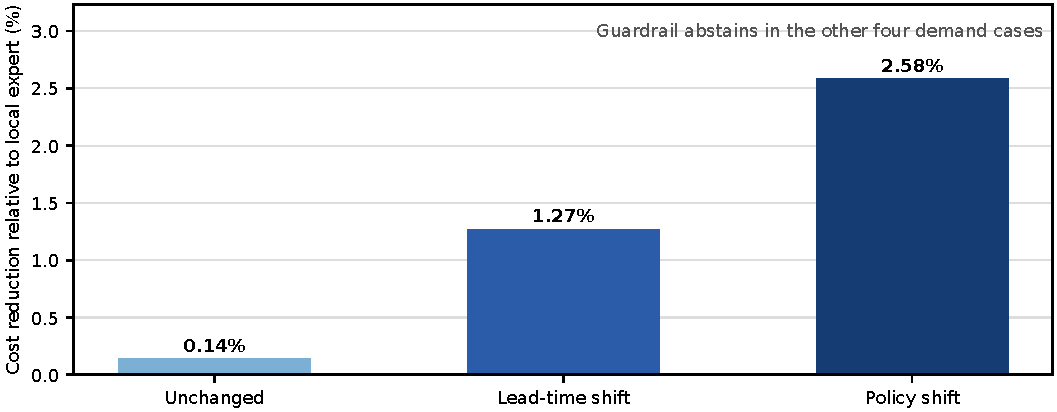
\includegraphics[width=.92\linewidth]{igrb_policy_savings.pdf}
\caption{Closed-loop cost reduction of the guarded IGRB policy relative to the guarded local-expert policy in correlated demand. Other cases are omitted because both guardrails abstain.}\label{fig:policy}
\end{figure}
The operational effect is smallest in the unchanged condition: cost falls by about 70 units out of 50,907 while fill rate rises from 0.5796 to 0.5804. This 0.14\% change is not presented as a large managerial saving. Its value is diagnostic: the complete forecast--selection--allocation pipeline avoids adding cost after the guardrail authorizes action. Under the lead-time shift the gap is about 923 units and fill rate rises by 0.0050; under the policy shift the gap is about 1,925 units and fill rate rises by 0.0102. These paired directional changes suggest more effective allocation of scarce emergency capacity in this simulated regime. They do not show that severity estimation is uniformly better, nor do they establish the optimality of the emergency rule.
\FloatBarrier
